\documentclass[11pt,a4paper]{ctexart}
\usepackage[margin=1.85cm]{geometry}
\usepackage{amsmath,amssymb,bm}
\usepackage{booktabs,graphicx,xcolor,hyperref,array,float}
\hypersetup{colorlinks=true,linkcolor=blue,urlcolor=blue}
\setlength{\parindent}{2em}
\setlength{\parskip}{0.22em}
\title{原始论文代码与当前最新 InEKF 的公平效果对比}
\author{统一事件计划、隔离计时边界与可视化验证}
\date{2026年7月24日}

\begin{document}
\maketitle

\section{对比目标与结论}

本入口比较论文作者公开的原始 InEKF 源码与当前
\texttt{task03\_compiled} 完整生产路径。两者处理相同 IMU 和 UWB 事件，
正式计时不包含数据加载、滤波器构造、JIT、历史记录、误差计算和绘图。

在 const1 前 30 s 数据上，四轮单线程 AB/BA 交替回放的耗时中位数为
$7.998309$ s 和 $0.235335$ s：
\begin{equation}
 \boxed{
 S_{\mathrm{direct}}
 =\frac{\operatorname{median}(T_{\mathrm{author}})}
 {\operatorname{median}(T_{\mathrm{latest}})}
 =33.9869
 },\qquad
 \Delta T=-97.0577\%.
\end{equation}
每轮均执行 30,267 次 IMU 预测和 14,289 次 UWB 更新，没有通过降采样、
冻结偏置、降低维数或丢弃量测获得加速。

\section{与论文递推的数学对照}

论文的右不变 15 维误差状态可写为
\begin{equation}
 \delta x=
 [\delta\theta,\delta v,\delta p,\delta b_g,\delta b_a]
 \in\mathbb{R}^{15}.
\end{equation}
两套实现都执行同一类预测和标量 TDoA 更新：
\begin{align}
 \hat X_{k+1}^{-}&=f(\hat X_k^{+},u_k,\Delta t_k),\\
 P_{k+1}^{-}&=\Phi_kP_k^{+}\Phi_k^{\mathsf T}+Q_{d,k},\\
 r_j&=y_j-h_j(\hat X^-),\qquad
 S_j=H_jP^-H_j^{\mathsf T}+R_j,\\
 \mathrm{NIS}_j&=\frac{r_j^2}{S_j},\qquad
 \delta x_j=P^-H_j^{\mathsf T}S_j^{-1}r_j.
\end{align}
当前版本保留 float64、全部 15 个状态、每个 IMU 间隔的协方差传播和全部 UWB
量测。固定尺寸编译只改变执行映射：
\begin{equation}
 \mathcal K_{\mathrm{Python}}
 (e_i,\hat X,P,b)
 \longrightarrow
 \mathcal K_{\mathrm{compiled}}
 (e_i,\hat X,P,b),
\end{equation}
不改变滤波递推。本轮新增的无历史计时模式满足
\begin{equation}
 (\hat X_N,P_N,N_{\mathrm{uwb}},N_{\mathrm{reject}})
 \quad\text{保持计算，}\quad
 \{\hat X_i,P_i,\mathrm{NIS}_i\}_{i=1}^{N}\quad\text{不写入输出缓冲区}.
\end{equation}
因此它减少的是基准测量污染，而不是减少算法工作量；完整曲线由计时外的独立回放
生成。

\section{公平计时边界}

令 $\mathcal E$ 表示预计算且哈希固定的事件计划，$F_v$ 为版本 $v$ 的滤波器：
\begin{equation}
 T_v=
 t\!\left(F_v(\mathcal E;\,\mathrm{history}=0)\right).
\end{equation}
正式测量遵循：
\begin{itemize}
 \item 两边共享 $\mathcal E$，并断言预测和 UWB 处理计数相等；
 \item 数值库线程数为 1，正式区间关闭 Python GC；
 \item 先预热，再按 AB/BA 顺序交替测量，报告中位数、MAD 和逐轮配对比值；
 \item 原作者备份只读导入，其 commit 和源码 SHA-256 写入 JSON；
 \item 轨迹、RMSE 和 NIS 来自额外完整历史回放，不与速度数字混用。
\end{itemize}

\begin{table}[H]
\centering
\caption{30 s 公平回放计时}
\begin{tabular}{lrrr}
\toprule
指标 & 原作者源码 & 当前最新实现 & 对比\\
\midrule
中位数/s & 7.998309 & 0.235335 & 33.9869x\\
MAD/s & 0.030330 & 0.006429 & -\\
最小值/s & 7.898692 & 0.225013 & -\\
最大值/s & 8.036066 & 0.241969 & -\\
\bottomrule
\end{tabular}
\end{table}

\section{精度结果与风险-回报}

\begin{table}[H]
\centering
\caption{30 s 效果指标；负号表示误差减小}
\begin{tabular}{lrrr}
\toprule
指标 & 原作者源码 & 当前最新实现 & 相对变化\\
\midrule
位置 RMSE/m & 0.116266 & 0.107016 & $-7.956\%$\\
速度 RMSE/(m/s) & 0.076748 & 0.072891 & $-5.025\%$\\
姿态测地 RMSE/rad & 0.054714 & 0.157598 & $+188.040\%$\\
yaw RMSE/rad & 0.052949 & 0.157491 & $+197.441\%$\\
UWB 拒绝数 & 0/14,289 & 0/14,289 & 相同\\
\bottomrule
\end{tabular}
\end{table}

位置和速度有所改善，但姿态和 yaw 的 30 s RMSE 明显变差。当前版本为全圆未知
航向使用 2 rad 保守先验，而本条数据的真实初始 yaw 恰好接近 $0^\circ$；
因此当前版本产生约 24 s 的初始 yaw 收敛瞬态。该选择避免大初始航向误差时的
过度自信，是可观测性稳健性与零初差短时 RMSE 之间的真实权衡，不能把本表概括为
“全部精度提升”。编译路径本身与 Python \texttt{proposed} 已通过逐元素等价测试。

\begin{figure}[H]
\centering
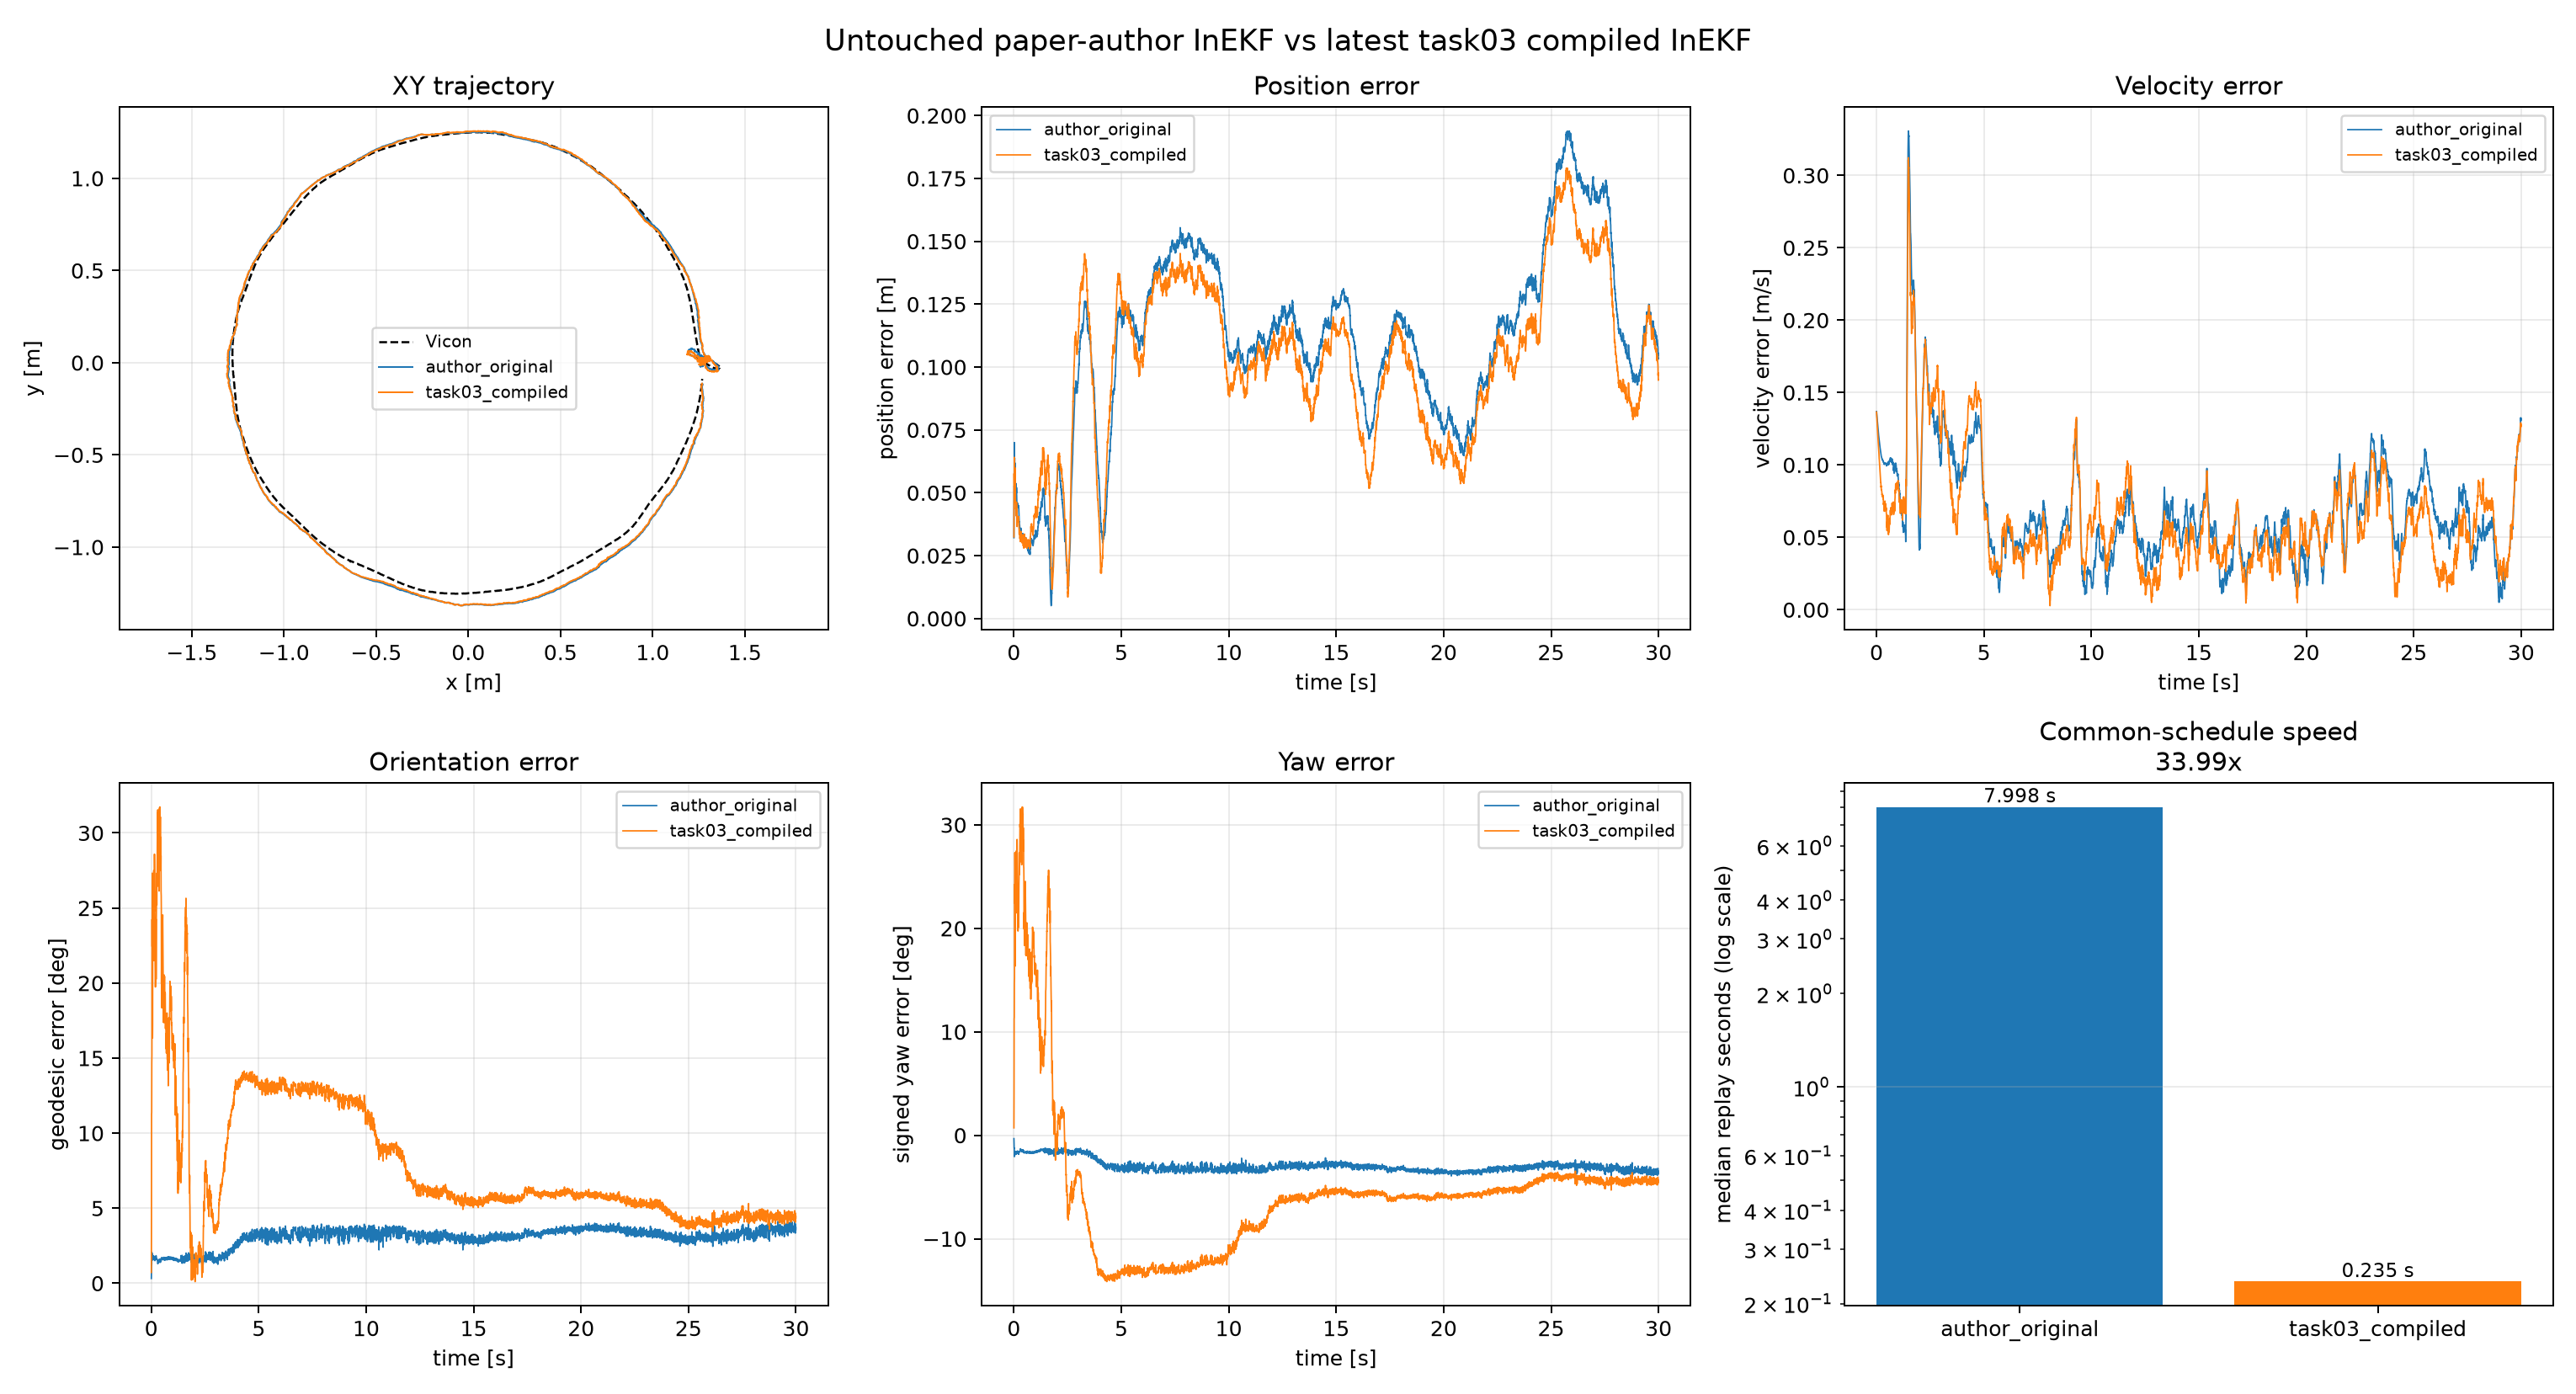
\includegraphics[width=0.90\textwidth]{../imu-uwb-inekf/results/fair_author_original_vs_latest_const1_30s/comparison.png}
\caption{轨迹、位置/速度/姿态/yaw 误差与公平回放耗时}
\end{figure}

\begin{figure}[H]
\centering
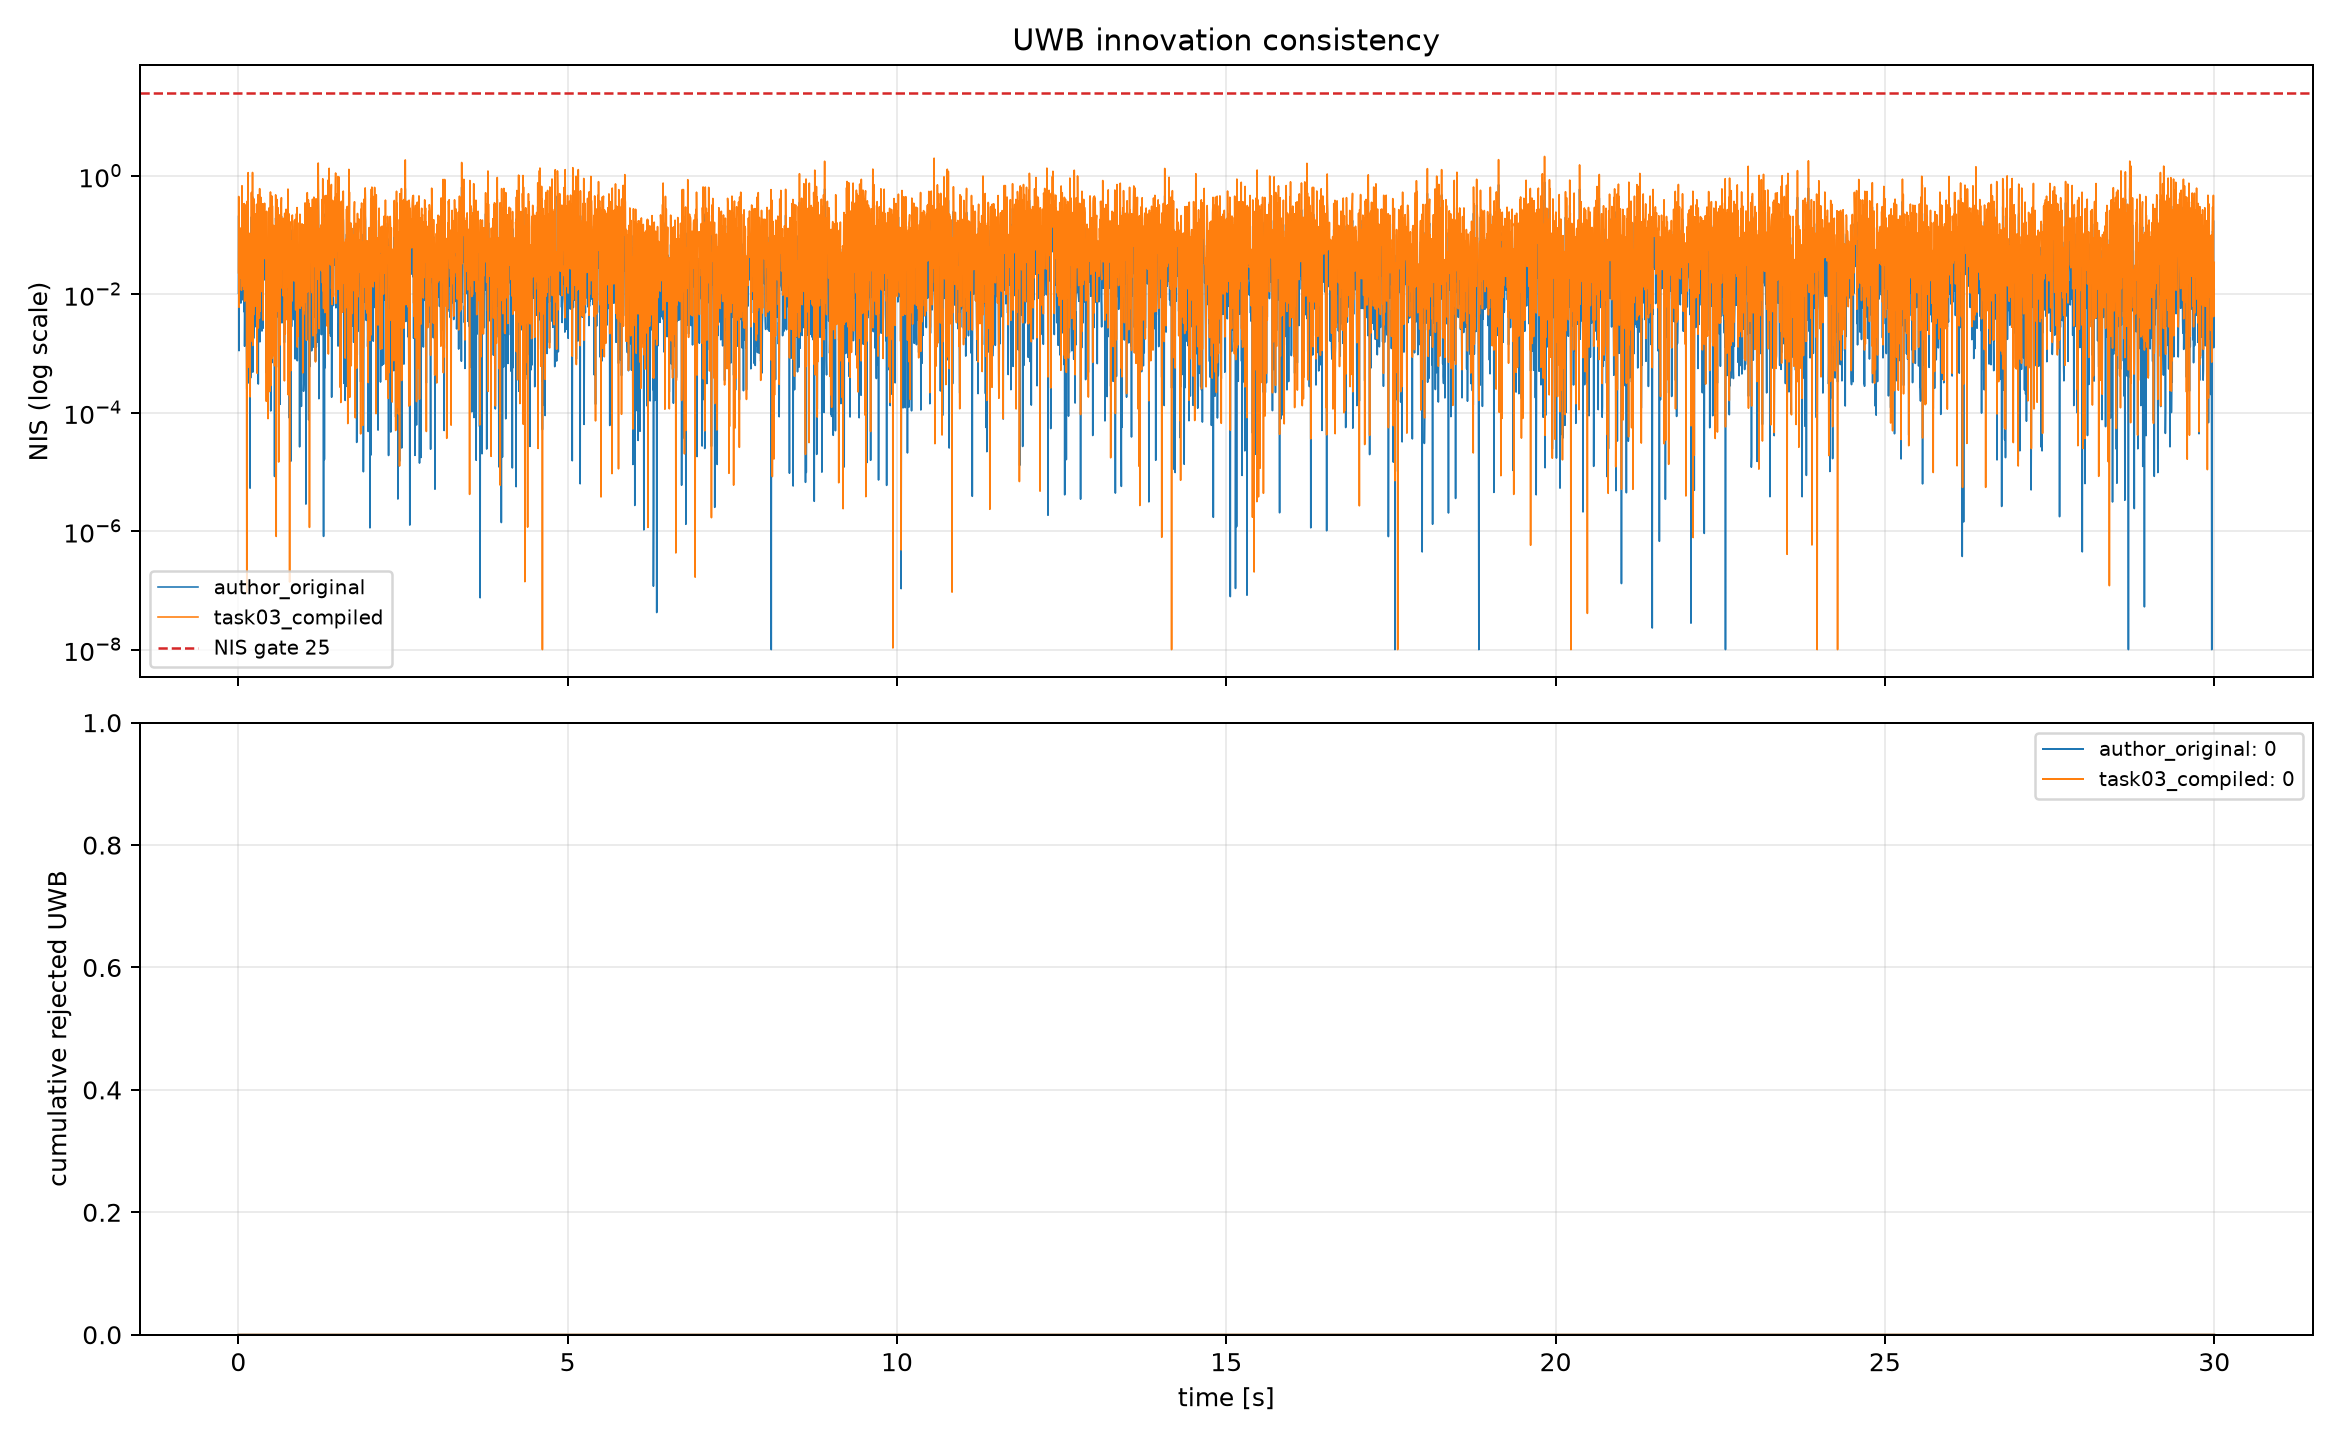
\includegraphics[width=0.76\textwidth]{../imu-uwb-inekf/results/fair_author_original_vs_latest_const1_30s/nis_and_rejections.png}
\caption{UWB NIS 与累计拒绝数；门限为 25，两边均无拒绝}
\end{figure}

\section{适用边界}

该结果证明的是指定 Windows 主机、Conda 环境、单线程和该 30 s 数据段上的离线
回放效果，不是目标嵌入式平台的 WCET，也不能外推全部星座、航向和机动条件。
旧的“作者源码对 proposed”与“proposed 对编译核”采用不同的计时边界，因此不能
机械相乘；应以本入口的直接测量为准。完整复现实验应保留 JSON 中的事件计划哈希、
源码哈希、逐轮时间和曲线。

\end{document}
